%%%%%%%%%%%%%%%%%%%%%%%%%%%%%%%%%%%%%%%%%
% Jacobs Landscape Poster
% LaTeX Template
% Version 1.0 (29/03/13)
%
% Created by:
% Computational Physics and Biophysics Group, Jacobs University
% https://teamwork.jacobs-university.de:8443/confluence/display/CoPandBiG/LaTeX+Poster
% 
% Further modified by:
% Nathaniel Johnston (nathaniel@njohnston.ca)
%
% This template has been downloaded from:
% http://www.LaTeXTemplates.com
%
% License:
% CC BY-NC-SA 3.0 (http://creativecommons.org/licenses/by-nc-sa/3.0/)
%
%%%%%%%%%%%%%%%%%%%%%%%%%%%%%%%%%%%%%%%%%

%----------------------------------------------------------------------------------------
%	PACKAGES AND OTHER DOCUMENT CONFIGURATIONS
%----------------------------------------------------------------------------------------

\documentclass[final]{beamer}

\usepackage[scale=1.2]{beamerposter} % Use the beamerposter package for laying out the poster

\usetheme{confposter} % Use the confposter theme supplied with this template


\setbeamercolor{block title}{fg=dblue,bg=dblue!10} % Colors of the block titles
\setbeamercolor{block body}{fg=black,bg=dblue!10} % Colors of the body of blocks
\setbeamercolor{block alerted title}{fg=white,bg=dblue!70} % Colors of the highlighted block titles
\setbeamercolor{block alerted body}{fg=black,bg=dblue!10} % Colors of the body of highlighted blocks
% Many more colors are available for use in beamerthemeconfposter.sty

%-----------------------------------------------------------
% Define the column widths and overall poster size
% To set effective sepwid, onecolwid and twocolwid values, first choose how many columns you want and how much separation you want between columns
% In this template, the separation width chosen is 0.024 of the paper width and a 4-column layout
% onecolwid should therefore be (1-(# of columns+1)*sepwid)/# of columns e.g. (1-(4+1)*0.024)/4 = 0.22
% Set twocolwid to be (2*onecolwid)+sepwid = 0.464
% Set threecolwid to be (3*onecolwid)+2*sepwid = 0.708

\newlength{\sepwid}
\newlength{\onecolwid}
\newlength{\twocolwid}
\newlength{\threecolwid}
\setlength{\paperwidth}{48in} % A0 width: 46.8in
\setlength{\paperheight}{36in} % A0 height: 33.1in
\setlength{\sepwid}{0.024\paperwidth} % Separation width (white space) between columns
\setlength{\onecolwid}{0.3\paperwidth} % Width of one column
\setlength{\twocolwid}{0.464\paperwidth} % Width of two columns
\setlength{\threecolwid}{0.708\paperwidth} % Width of three columns
\setlength{\topmargin}{-0.5in} % Reduce the top margin size
%-----------------------------------------------------------

\usepackage{graphicx}  % Required for including images
\usepackage{minted}
\usepackage{booktabs} % Top and bottom rules for tables

%----------------------------------------------------------------------------------------
%	TITLE SECTION 
%----------------------------------------------------------------------------------------

\title{PHASM: Parallel Hardware viA Surrogate Models} % Poster title

\author{Nathan Brei, Cissie Mei, Kishan Rajput, David Lawrence} % Author(s)

\institute{Jefferson Lab} % Institution(s)

%----------------------------------------------------------------------------------------

\begin{document}

\addtobeamertemplate{block end}{}{\vspace*{2ex}} % White space under blocks
\addtobeamertemplate{block alerted end}{}{\vspace*{2ex}} % White space under highlighted (alert) blocks

\setlength{\belowcaptionskip}{1ex} % White space under figures
\setlength\belowdisplayshortskip{1ex} % White space under equations

\begin{frame}[fragile,t] % The whole poster is enclosed in one beamer frame

\begin{columns}[t] % The whole poster consists of three major columns, the second of which is split into two columns twice - the [t] option aligns each column's content to the top

\begin{column}{0.5\sepwid}\end{column} % Empty spacer column

\begin{column}{\onecolwid} % The first column


\begin{block}{Motivation}
\textbf{PHASM simplifies and formalizes the process of training a neural net surrogate model to mimic and replace an arbitrary piece of existing ('legacy') code.}


A neural net trained to mimic an existing numerical algorithm is just another numerical algorithm. However:
\begin{itemize}
\item Neural net surrogates have different time and space complexity. This gives us fast simulations and inverse simulations.

\item Unlike other modelling techniques, neural nets can sidestep the \emph{curse of dimensionality}. This makes surrogate models feasible for a much wider class of algorithms than in the past.

\item They can have much higher internal parallelism than the original algorithms, so they can run efficiently on \emph{heterogeneous hardware} such as GPUs, TPUs, and FPGAs. The transformation is often automatic.

Modern data centers are investing heavily in heterogeneous hardware, but many important codebases are unable to take advantage of it without undergoing a costly rewrite. Neural net surrogate models could mitigate this.
\end{itemize}
\end{block}

\begin{figure}
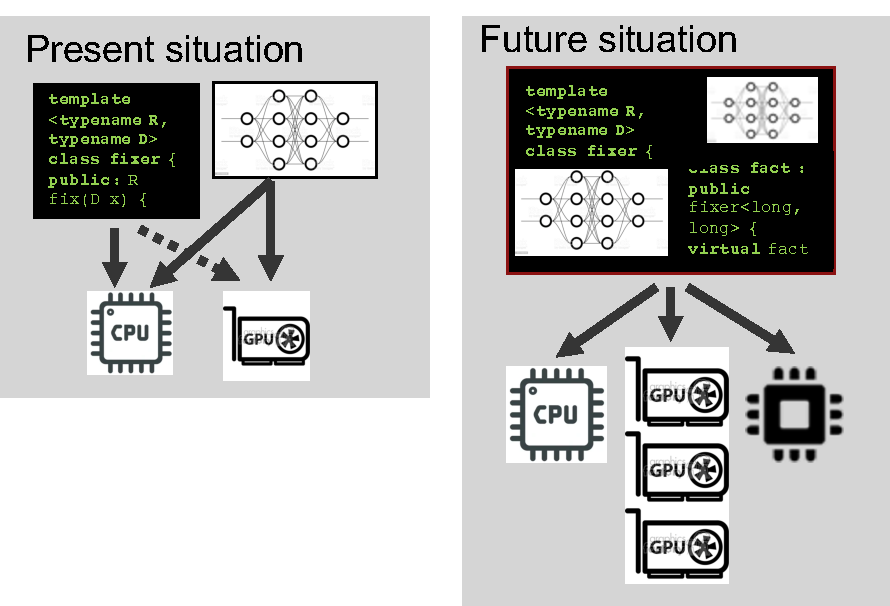
\includegraphics[width=0.6\linewidth]{cartoon2.pdf}
\end{figure}


\begin{block}{Strategic goals}
\begin{enumerate}
\item Create an interactive tool for testing surrogate models empirically and rapidly, without recompiling. Analogous to a debugger: Pause execution of the program and present the user with options such as: profile a function, rewrite the binary to replace a function with a surrogate, tune the surrogate’s hyperparameters, capture training data, etc.


\item Pieces of this tool should be usable on their own and should help productionize ML models around the lab. We want to make it easy to integrate best-in-class ML tools into established codebases. 


\item This opens up new research opportunities into mixing neural nets with numerical methods, and embedding domain knowledge and UQ. Example: Synthetic generation of training data using static analysis/fuzzing. 

\end{enumerate}
\end{block}



%------------------------------------------------

%----------------------------------------------------------------------------------------

\end{column} % End of the first column

\begin{column}{0.5\sepwid}\end{column} % Empty spacer column

\begin{column}{\onecolwid} % Begin a column which is two columns wide (column 2)




\begin{block}{Surrogate API}

This tool provides a high-level interface for specifying the input variables, their bounds, and the model parameters. Meanwhile it abstracts away the work of integrating a ML framework, capturing training samples, choosing additional training samples, training the model, loading and storing the trained model, and switching between the original function and the surrogate. 

It uses \emph{profunctor optics} to perform simple and effective two-way data transformation between C++ types and tensors. Currently supports primitives, arrays, structures, and unions. Correctly handles nested datatypes, e.g. an array containing a struct containing an array of doubles translates to a 2D tensor of doubles, without writing any loops!

\end{block}



\begin{block}{Surrogate API example}
\begin{minted}[fontsize=\small]{cpp}

double f(double x, double y, double z) {
    return 3*x*x + 2*y + z;
}

phasm::Surrogate f_surrogate = phasm::SurrogateBuilder()
        .set_model(std::make_shared<phasm::FeedForwardModel>())
        .local_primitive<double>("x", phasm::IN)
        .local_primitive<double>("y", phasm::IN)
        .local_primitive<double>("z", phasm::IN)
        .local_primitive<double>("retval", phasm::OUT)
        .finish();

double f_wrapper(double x, double y, double z) {
    double res = 0.0;
    f_surrogate.bind_original_function([&](){res = f(x,y,z);})
               .bind_all_callsite_vars(&x, &y, &z)
               .call();  // $PHASM_CALL_MODE controls this
}
\end{minted}
\end{block}


\begin{block}{Model variable discovery tool}

This tool takes a function and identifies all of its inputs and outputs (global variables, nested structures, pointers, etc).
It reports the shape and size of the memory being moved, and generates the optics that convert the data to and from tensors. This novel idea effectively turns an impure function of rich nested datatypes into a pure function of tensors, opening the door to property-based testing, numerical sensitivity/stability analyses, etc.


It works by doing a dynamic binary analysis (built on Intel PIN) to intercept and log memory accesses and allocations, similar to valgrind memcheck. It then uses DWARF debugging data to resolve variable names and types. It currently supports primitives, arrays, and structures/classes. 

\end{block}



\end{column} % End of the second column

\begin{column}{0.5\sepwid}\end{column} % Empty spacer column

\begin{column}{\onecolwid} % The third column


\begin{block}{Performance analysis playbook}
This tool qualitatively predicts, for an arbitrary function, whether and when a surrogate model would run effectively on heterogeneous hardware.
We systematize the analysis into a step-by-step playbook, detailing which tools to use, which metrics to capture, and how to interpret them. The goal is to make it realistic for researchers to do a thorough analysis before writing any code. 

We currently use a roofline analysis coupled with Amdahl's and Gustavsson's Laws to predict the performance of the surrogate model.

\end{block}



\begin{figure}
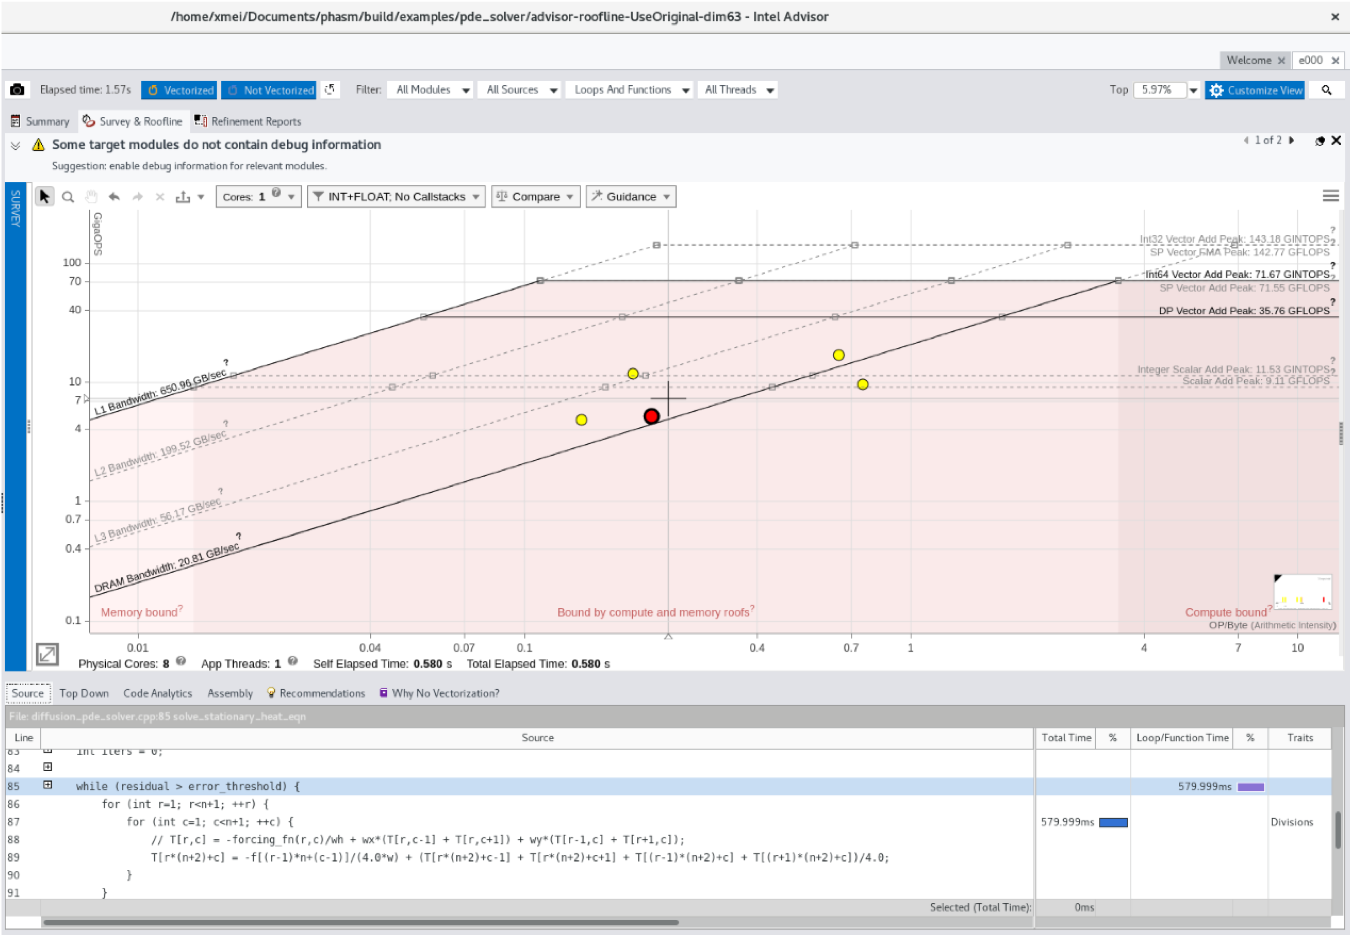
\includegraphics[width=0.8\linewidth]{roofline.png}
\end{figure}


\begin{block}{Next steps}

\begin{description}
\item[Multiple ML backends]\ Rearchitect the Surrogate API to support multiple ML frameworks via dynamically loaded backends, similar to how GlueX+JANA uses plugins.

\item[MLFlow integration]\ MLFlow is a model repository that handles versioning, annotating, and sharing of trained machine learning models. It is a research priority of JLab’s data science department.

\item[Static analysis]\ Experiment with performing a static code analysis for model variable discovery instead, using ROSE or LLVM/clang. 

\item[Validate using Geant4]\ Use PHASM to demonstrate effective subevent-level parallelism within Geant4. Create a surrogate for a calorimeter detector simulation kernel. This kernel has already been calculated to perform well under GPU offloading, but no CUDA port has been written.

\end{description}

\end{block}



\begin{block}{References}
\begin{itemize}
\item Code: \href{http://www.github.com/nathanwbrei/phasm}{http://www.github.com/nathanwbrei/phasm}
\item Email: \href{mailto:nbrei@jlab.org}{nbrei@jlab.org}
\end{itemize}
\end{block}



%----------------------------------------------------------------------------------------

\end{column} % End of the third column

\end{columns} % End of all the columns in the poster


\footnotesize{This material is based upon work supported by the U.S. Department of Energy, Office of Science, Office of Nuclear Physics under contract DE-AC05-06OR23177. This project is funded by Jefferson Lab LDRD project LD2213.}

\end{frame}

\end{document}
